\subsection{Phân tích OLAP}

OLAP (Online Analytical Processing) \cite{chaudhuri1997} là kỹ thuật trung tâm để khai thác Kho dữ liệu theo nhiều chiều khác nhau. Trên \texttt{gold.fact\_market\_daily} kết hợp với 3 bảng chiều (\texttt{dim\_date}, \texttt{dim\_coin}, \texttt{dim\_category}), nhóm xây dựng 3 view phân tích sẵn sàng cho dashboard và 3 báo cáo trực quan tổng hợp.

\subsubsection{Các view OLAP cốt lõi}

\begin{itemize}
    \item \texttt{gold.v\_weekly\_return\_by\_category}: Trung bình \texttt{return\_pct} theo tuần và \texttt{category\_name}, dùng cho biểu đồ heatmap so sánh hiệu suất giữa nhóm L1, L2, Meme và Payment.
    \item \texttt{gold.v\_volume\_leaderboard}: Bảng xếp hạng thanh khoản (\texttt{volume\_usd}) toàn bộ kỳ, có \texttt{volume\_rank} chốt mỗi ngày.
    \item \texttt{gold.v\_top\_anomalies}: Danh sách các phiên có \texttt{is\_anomaly = TRUE} ($|z\_score| > 2$), hỗ trợ cảnh báo sớm các sự kiện cực đoan.
\end{itemize}

\subsubsection{Diễn biến giá tổng hợp (Combined Price Trend)}

\begin{figure}[H]
    \centering
    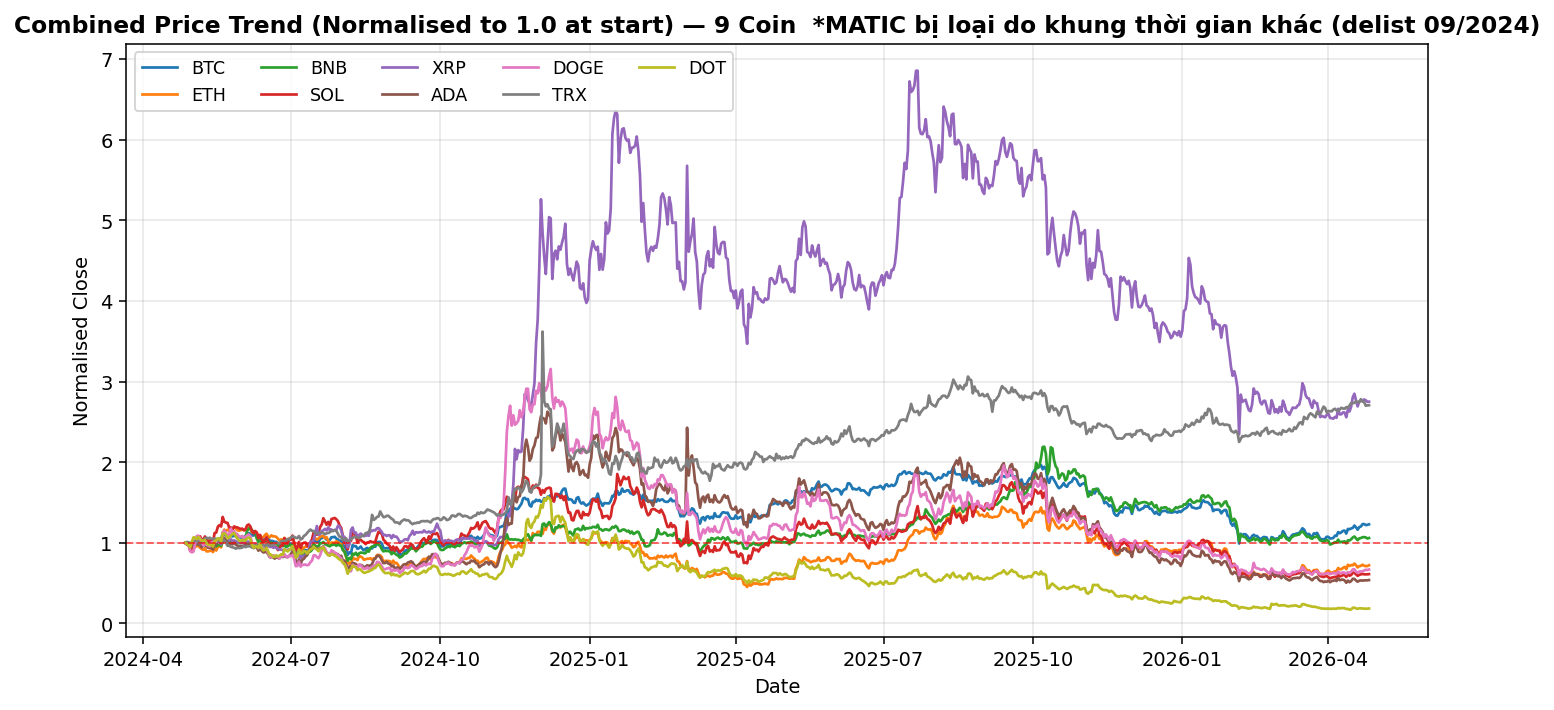
\includegraphics[width=\linewidth]{Images/OLAP/01_combined_price_trend.png}
    \caption{Diễn biến giá đóng cửa của 10 coin (chuẩn hoá về 1.0 ở đầu kỳ)}
    \label{fig:olap_price_trend}
\end{figure}

Biểu đồ \ref{fig:olap_price_trend} chuẩn hoá giá đóng cửa về mức 1.0 vào ngày bắt đầu mẫu (27/04/2024) để có thể so sánh trực tiếp hiệu suất tích luỹ giữa 9 coin. \textit{MATIC bị loại khỏi biểu đồ tổng hợp này do khung thời gian khác biệt (Binance đã delist sau khi Polygon rebrand sang POL vào 09/2024).} Có thể quan sát rõ:
\begin{itemize}
    \item \textbf{Nhóm dẫn dắt:} BTC, BNB và TRX duy trì xu hướng tăng tương đối ổn định, kết thúc kỳ với mức tăng dương đáng kể.
    \item \textbf{Nhóm phân hoá mạnh:} XRP có cú bứt phá ngoạn mục cuối 2024 (sau pha tăng vọt liên quan ETF), trong khi DOT, ADA, MATIC liên tục downtrend, mất phần lớn giá trị so với đầu kỳ.
    \item \textbf{Tương quan ngành rõ rệt:} Pha sụt giảm chung cuối Q1/2025 thể hiện đặc tính đồng pha cao của crypto -- một sự kiện vĩ mô (lãi suất, tin tức quy định) tác động đến gần như toàn thị trường.
\end{itemize}

\subsubsection{Xếp hạng khối lượng giao dịch năm 2025}

\begin{figure}[H]
    \centering
    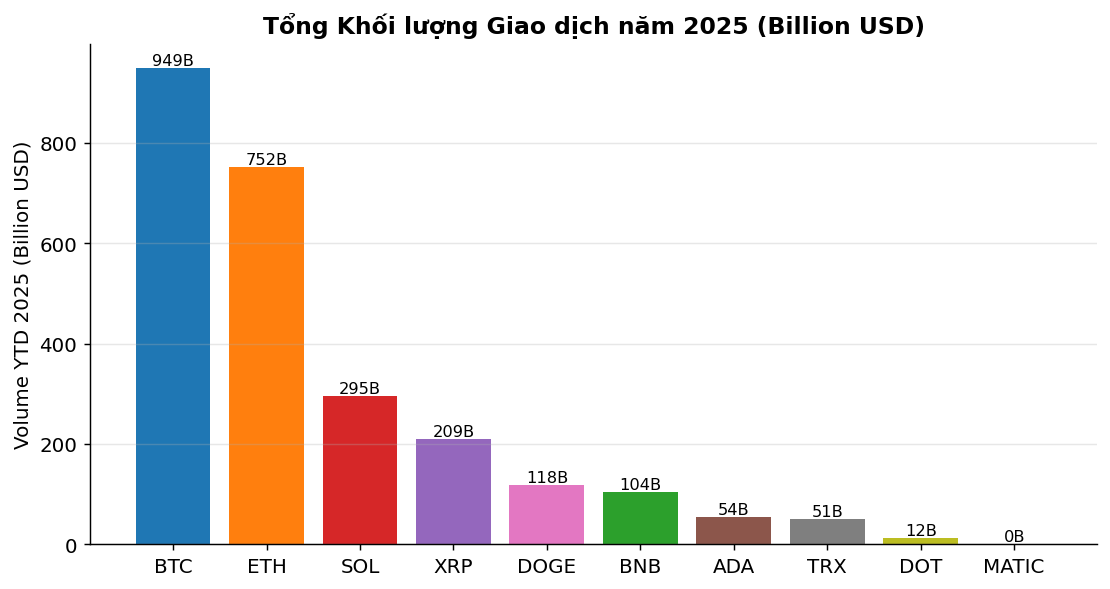
\includegraphics[width=\linewidth]{Images/OLAP/02_combined_volume_2025.png}
    \caption{Tổng khối lượng giao dịch năm 2025 (Billion USD) -- xếp hạng top 10 coin}
    \label{fig:olap_volume_2025}
\end{figure}

Biểu đồ \ref{fig:olap_volume_2025} sử dụng aggregation \texttt{SUM(volume\_usd)} từ 01/01/2025 đến hết kỳ, nhóm theo \texttt{symbol}. Kết quả cho thấy sự phân hoá thanh khoản cực mạnh:
\begin{itemize}
    \item \textbf{BTC vẫn áp đảo} với khối lượng giao dịch quy đổi USD vượt trội, củng cố vị thế tài sản số ``vàng kỹ thuật số''.
    \item \textbf{ETH và SOL} chia sẻ vị trí dẫn dắt nhóm Layer-1 thay thế.
    \item \textbf{Nhóm còn lại} (ADA, DOT, MATIC, TRX, ...) có thanh khoản thấp hơn 1--2 bậc magnitude, phản ánh xu hướng dòng tiền tập trung vào các coin có nền tảng vững chắc.
\end{itemize}
Đây cũng là cơ sở cho chiến lược ``follow the volume'' khi phát hiện breakout/breakdown -- chỉ những tín hiệu giá trên BTC/ETH/SOL kèm volume spike mới đáng tin cậy.

\subsubsection{Heatmap lợi suất tháng}

\begin{figure}[H]
    \centering
    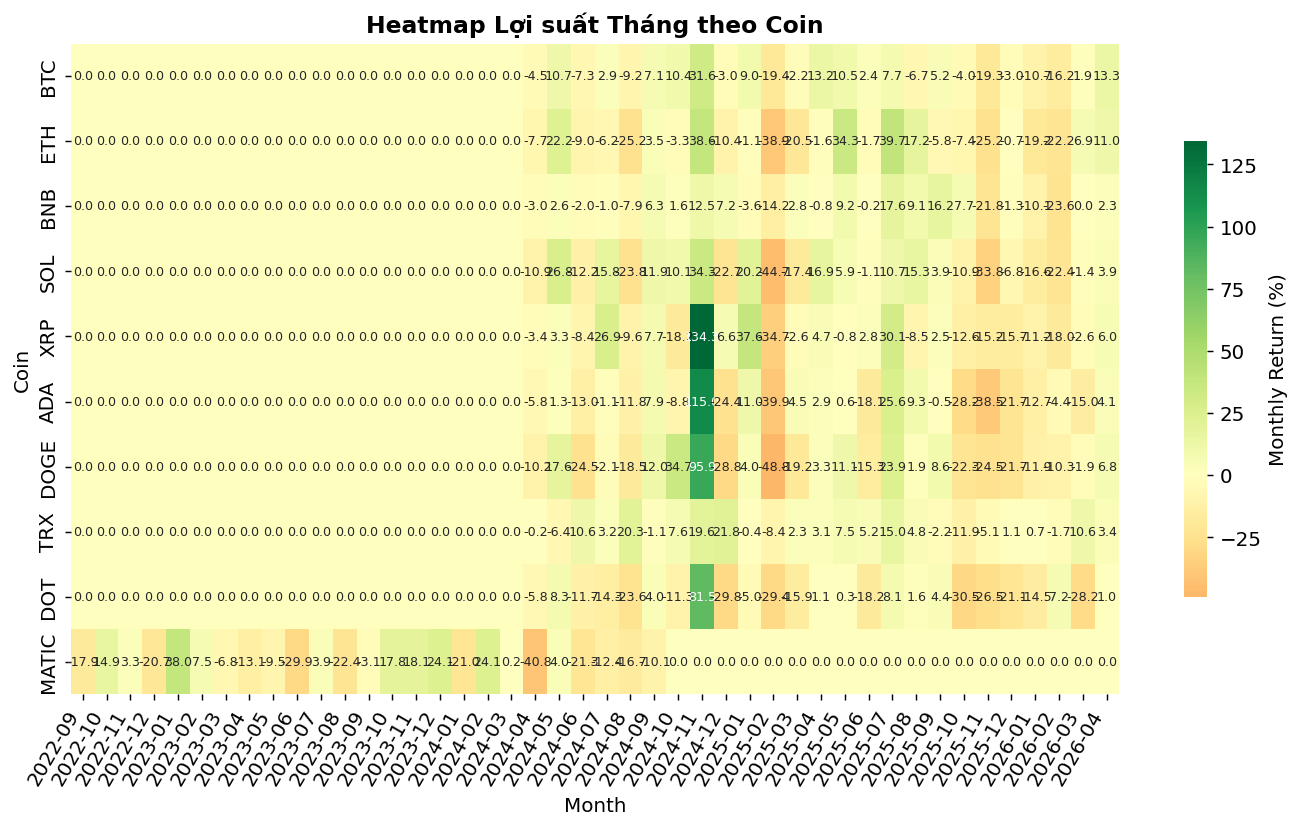
\includegraphics[width=\linewidth]{Images/OLAP/03_combined_heatmap_price.png}
    \caption{Heatmap lợi suất tháng (cumulative log-return $\times 100$) theo coin}
    \label{fig:olap_heatmap}
\end{figure}

Biểu đồ \ref{fig:olap_heatmap} là dạng pivot trục Coin $\times$ Month với giá trị là tổng \texttt{log\_return} theo tháng (chuyển sang \%). Màu xanh lá biểu thị tháng tăng giá, màu đỏ biểu thị tháng giảm. Đây chính là một thao tác OLAP \textbf{Pivot/Rotate} điển hình. Quan sát:
\begin{itemize}
    \item Các tháng có cú bùng nổ chung (cả cột màu xanh sáng) thường trùng với các sự kiện vĩ mô tích cực: ETF được phê duyệt, Bitcoin halving, Fed cắt lãi suất.
    \item Các tháng giảm sâu đồng loạt (cả cột màu đỏ đậm) trùng với các sự kiện rủi ro hệ thống.
    \item DOGE và XRP thường xuyên có biên độ tháng lớn nhất (cả tăng lẫn giảm), khẳng định đặc tính ``high-volatility / event-driven'' của hai mã này.
\end{itemize}

Heatmap này cho phép thực hiện thao tác \textbf{Drill-down} đơn giản: từ một ô có biến động bất thường, người dùng có thể truy vấn xuống cấp ngày để tìm phiên cụ thể, sau đó cross-reference với \texttt{v\_top\_anomalies} để tìm nguyên nhân.

\subsubsection{Tổng hợp các thao tác OLAP áp dụng}

\begin{itemize}
    \item \textbf{Slice:} Lọc theo một ngày (\texttt{WHERE date\_id = 20250115}) hoặc một coin.
    \item \textbf{Dice:} Cắt theo tổ hợp nhiều chiều, ví dụ chỉ xem nhóm L1 trong Q2/2025.
    \item \textbf{Drill-down / Roll-up:} Từ mức năm $\rightarrow$ quý $\rightarrow$ tháng $\rightarrow$ ngày qua \texttt{dim\_date}.
    \item \textbf{Pivot:} Xoay trục như Heatmap Coin $\times$ Month ở hình \ref{fig:olap_heatmap}.
\end{itemize}
